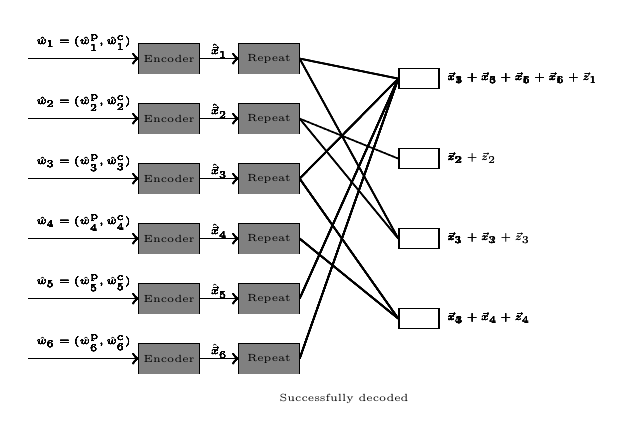
\begin{tikzpicture}
\def\horzgap{0.75in}; %Horizontal gap between nodes/levels
\def \gapVN{0.3in}; %vertical gap between nodes
\def \gapCN{0.4in}; %Horizontal gap between nodes
\def\fsize{\tiny}
\def\fac{0.75}
\def\lw{0.2mm}

\def\nodewidth{0.1in}; 
\def\nodewidthA{0.2in};
\def \edgewidth{15ex}; 
\def\ext{0.5in};


\tikzstyle{check} = [rectangle, draw,line width=\lw, inner sep=0mm, minimum height=\nodewidth, minimum width=2*\nodewidth]
\tikzstyle{block} = [rectangle, draw, line width=\lw, inner sep=0mm,  minimum height=\nodewidthA, minimum width=2*\nodewidthA]
\tikzstyle{bit} = [circle, draw, line width=\lw, inner sep=0mm,  minimum size=\nodewidthA]
\tikzstyle{blockuncover} = [rectangle, draw=none, fill=gray, line width=\lw, inner sep=0mm,  minimum height=\nodewidthA, minimum width=2*\nodewidthA]

 \def\moveX {1.8*\nodewidth};
\def\moveXA {2*\nodewidth};



\onslide<1>{             

\foreach \vn in {1,...,6}{
\node[block,scale=\fac] (vn\vn) at (0,-\vn*\gapVN) {\tiny{Repeat}};
\path (vn\vn)++(-\ext,0) node[scale=\fac,block] (vna\vn) {\tiny{Encoder}};
\draw[->,line width=\lw] (vna\vn.east)--node[midway,above,scale=\fac, inner sep=0mm] {\fsize{$\vec{x}_{\vn}$}} (vn\vn.west);
\draw[<-, line width=\lw] (vna\vn.west)--node[midway, above,scale=\fac]{\fsize{$w_{\vn} =(w_{\vn}^{\mathrm{p}}, w_{\vn}^{\mathrm{c}})$}}+(-1.1*\ext,0);
}

\foreach \cn in {1,...,4}{
\node[check] (cn\cn) at (\horzgap,-\cn*\gapCN) {};
}

\draw[line width=\lw] (vn4.east)--(cn4.west);
\draw[line width=\lw] (vn3.east)--(cn4.west);

\draw[line width=\lw] (vn2.east)--(cn3.west);
\draw[line width=\lw] (vn1.east)--(cn3.west);

\draw[line width=\lw] (vn2.east)--(cn2.west);

\draw[line width=\lw] (vn1.east)--(cn1.west);
\draw[line width=\lw] (vn3.east)--(cn1.west);
\draw[line width=\lw] (vn5.east)--(cn1.west);
\draw[line width=\lw] (vn6.east)--(cn1.west);


\node [scale=\fac,anchor=west] at (cn1.east) {\fsize{$\vec{x}_1+\vec{x}_3+\vec{x}_5+\vec{x}_6+\vec{z}_1$}};
\node [scale=\fac,anchor=west] at (cn2.east) {\fsize{$\vec{x}_2+\vec{z}_2$}};
\node [scale=\fac,anchor=west] at (cn3.east) {\fsize{$\vec{x}_1+\vec{x}_2+\vec{z}_3$}};
\node [scale=\fac,anchor=west] at (cn4.east) {\fsize{$\vec{x}_3+\vec{x}_4+\vec{z}_4$}};
}

%%-----------------------*(&^#@$^&*(^%$^&*(&^--------------------------------------------------------------------
%Dotted x_2

\onslide<2>{

\foreach \vn in {1,3,4,5,6}{
\node[block,scale=\fac] (vn\vn) at (0,-\vn*\gapVN) {\tiny{Repeat}};
\path (vn\vn)++(-\ext,0) node[scale=\fac,block] (vna\vn) {\tiny{Encoder}};
\draw[->,line width=\lw] (vna\vn.east)--node[midway,above,scale=\fac, inner sep=0mm] {\fsize{$\vec{x}_{\vn}$}} (vn\vn.west);
\draw[<-, line width=\lw] (vna\vn.west)--node[midway, above,scale=\fac]{\fsize{$w_{\vn} =(w_{\vn}^{\mathrm{p}}, w_{\vn}^{\mathrm{c}})$}}+(-1.1*\ext,0);
}


\foreach \vn in {2}{
\node[blockuncover,scale=\fac] (vn\vn) at (0,-\vn*\gapVN) {\tiny{Repeat}};
\path (vn\vn)++(-\ext,0) node[scale=\fac,blockuncover] (vna\vn) {\tiny{Encoder}};
\draw[->,line width=\lw] (vna\vn.east)--node[midway,above,scale=\fac, inner sep=0mm] {\fsize{$\hat{\vec{x}}_{\vn}$}} (vn\vn.west);
\draw[<-, line width=\lw] (vna\vn.west)--node[midway, above,scale=\fac]{\fsize{$\hat{w}_{\vn} =(\hat{w}_{\vn}^{\mathrm{p}},\hat{w}_{\vn}^{\mathrm{c}})$}}+(-1.1*\ext,0);
}

\foreach \cn in {1,...,4}{
\node[check] (cn\cn) at (\horzgap,-\cn*\gapCN) {};
}


\draw[line width=\lw] (vn4.east)--(cn4.west);
\draw[line width=\lw] (vn3.east)--(cn4.west);

\draw[line width=\lw] (vn2.east)--(cn3.west);
\draw[line width=\lw] (vn1.east)--(cn3.west);

\draw[line width=\lw, densely dotted] (vn2.east)--(cn2.west);

\draw[line width=\lw] (vn1.east)--(cn1.west);
\draw[line width=\lw] (vn3.east)--(cn1.west);
\draw[line width=\lw] (vn5.east)--(cn1.west);
\draw[line width=\lw] (vn6.east)--(cn1.west);

\node [scale=\fac,anchor=west] at (cn1.east) {\tiny{$\vec{x}_1+\vec{x}_3+\vec{x}_5+\vec{x}_6+\vec{z}_1$}};
\node [scale=\fac,anchor=west] at (cn2.east) {\tiny{$\vec{x}_2+\vec{z}_2$}};
\node [scale=\fac,anchor=west] at (cn3.east) {\tiny{$\vec{x}_1+\vec{x}_2+\vec{z}_3$}};
\node [scale=\fac,anchor=west] at (cn4.east) {\tiny{$\vec{x}_3+\vec{x}_4+\vec{z}_4$}};
}

%%----------------------------------^%$#@%^&*()_*&^%$#^&*------------------------------------
%%--Peeled x_2
\onslide<3>{

\foreach \vn in {1,3,4,5,6}{
\node[block,scale=\fac] (vn\vn) at (0,-\vn*\gapVN) {\tiny{Repeat}};
\path (vn\vn)++(-\ext,0) node[scale=\fac,block] (vna\vn) {\tiny{Encoder}};
\draw[->,line width=\lw] (vna\vn.east)--node[midway,above,scale=\fac, inner sep=0mm] {\fsize{$\vec{x}_{\vn}$}} (vn\vn.west);
\draw[<-, line width=\lw] (vna\vn.west)--node[midway, above,scale=\fac]{\fsize{$w_{\vn} =(w_{\vn}^{\mathrm{p}}, w_{\vn}^{\mathrm{c}})$}}+(-1.1*\ext,0);
}


\foreach \vn in {2}{
\node[blockuncover,scale=\fac] (vn\vn) at (0,-\vn*\gapVN) {\tiny{Repeat}};
\path (vn\vn)++(-\ext,0) node[scale=\fac,blockuncover] (vna\vn) {\tiny{Encoder}};
\draw[->,line width=\lw] (vna\vn.east)--node[midway,above,scale=\fac, inner sep=0mm] {\fsize{$\hat{\vec{x}}_{\vn}$}} (vn\vn.west);
\draw[<-, line width=\lw] (vna\vn.west)--node[midway, above,scale=\fac]{\fsize{$\hat{w}_{\vn} =(\hat{w}_{\vn}^{\mathrm{p}},\hat{w}_{\vn}^{\mathrm{c}})$}}+(-1.1*\ext,0);
}


\foreach \cn in {1,...,4}{
\node[check] (cn\cn) at (\horzgap,-\cn*\gapCN) {};
}


\draw[line width=\lw] (vn4.east)--(cn4.west);
\draw[line width=\lw] (vn3.east)--(cn4.west);

\draw[line width=\lw] (vn1.east)--(cn3.west);

\draw[line width=\lw] (vn1.east)--(cn1.west);
\draw[line width=\lw] (vn3.east)--(cn1.west);
\draw[line width=\lw] (vn5.east)--(cn1.west);
\draw[line width=\lw] (vn6.east)--(cn1.west);

\node [scale=\fac,anchor=west] at (cn1.east) {\tiny{$\vec{x}_1+\vec{x}_3+\vec{x}_5+\vec{x}_6+\vec{z}_1$}};
\node [scale=\fac,anchor=west] at (cn2.east) {\tiny{$\vec{z}_2$}};
\node [scale=\fac,anchor=west] at (cn3.east) {\tiny{$\vec{x}_1+\vec{z}_3$}};
\node [scale=\fac,anchor=west] at (cn4.east) {\tiny{$\vec{x}_3+\vec{x}_4+\vec{z}_4$}};
}

%%---------%^&*^%$#^&----------------------------
%%Dotted x_1
\onslide<4>{

\foreach \vn in {3,4,5,6}{
\node[block,scale=\fac] (vn\vn) at (0,-\vn*\gapVN) {\tiny{Repeat}};
\path (vn\vn)++(-\ext,0) node[scale=\fac,block] (vna\vn) {\tiny{Encoder}};
\draw[->,line width=\lw] (vna\vn.east)--node[midway,above,scale=\fac, inner sep=0mm] {\fsize{$\vec{x}_{\vn}$}} (vn\vn.west);
\draw[<-, line width=\lw] (vna\vn.west)--node[midway, above,scale=\fac]{\fsize{$w_{\vn} =(w_{\vn}^{\mathrm{p}}, w_{\vn}^{\mathrm{c}})$}}+(-1.1*\ext,0);
}


\foreach \vn in {1,2}{
\node[blockuncover,scale=\fac] (vn\vn) at (0,-\vn*\gapVN) {\tiny{Repeat}};
\path (vn\vn)++(-\ext,0) node[scale=\fac,blockuncover] (vna\vn) {\tiny{Encoder}};
\draw[->,line width=\lw] (vna\vn.east)--node[midway,above,scale=\fac, inner sep=0mm] {\fsize{$\hat{\vec{x}}_{\vn}$}} (vn\vn.west);
\draw[<-, line width=\lw] (vna\vn.west)--node[midway, above,scale=\fac]{\fsize{$\hat{w}_{\vn} =(\hat{w}_{\vn}^{\mathrm{p}},\hat{w}_{\vn}^{\mathrm{c}})$}}+(-1.1*\ext,0);
}


\foreach \cn in {1,...,4}{
\node[check] (cn\cn) at (\horzgap,-\cn*\gapCN) {};
}


\draw[line width=\lw] (vn4.east)--(cn4.west);
\draw[line width=\lw] (vn3.east)--(cn4.west);

\draw[line width=\lw, densely dotted] (vn1.east)--(cn3.west);
\draw[line width=\lw] (vn1.east)--(cn1.west);

\draw[line width=\lw] (vn3.east)--(cn1.west);
\draw[line width=\lw] (vn5.east)--(cn1.west);
\draw[line width=\lw] (vn6.east)--(cn1.west);


\node [scale=\fac,anchor=west] at (cn1.east) {\tiny{$\vec{x}_1+\vec{x}_3+\vec{x}_5+\vec{x}_6+\vec{z}_1$}};
\node [scale=\fac,anchor=west] at (cn2.east) {\tiny{$\vec{z}_2$}};
\node [scale=\fac,anchor=west] at (cn3.east) {\tiny{$\vec{x}_1+\vec{z}_3$}};
\node [scale=\fac,anchor=west] at (cn4.east) {\tiny{$\vec{x}_3+\vec{x}_4+\vec{z}_4$}};
}

%%----------------------------------^%$#@%^&*()_*&^%$#^&*------------------------------------
%%-peeled off x_1
\onslide<5>{

\foreach \vn in {3,4,5,6}{
\node[block,scale=\fac] (vn\vn) at (0,-\vn*\gapVN) {\tiny{Repeat}};
\path (vn\vn)++(-\ext,0) node[scale=\fac,block] (vna\vn) {\tiny{Encoder}};
\draw[->,line width=\lw] (vna\vn.east)--node[midway,above,scale=\fac, inner sep=0mm] {\fsize{$\vec{x}_{\vn}$}} (vn\vn.west);
\draw[<-, line width=\lw] (vna\vn.west)--node[midway, above,scale=\fac]{\fsize{$w_{\vn} =(w_{\vn}^{\mathrm{p}}, w_{\vn}^{\mathrm{c}})$}}+(-1.1*\ext,0);
}


\foreach \vn in {1,2}{
\node[blockuncover,scale=\fac] (vn\vn) at (0,-\vn*\gapVN) {\tiny{Repeat}};
\path (vn\vn)++(-\ext,0) node[scale=\fac,blockuncover] (vna\vn) {\tiny{Encoder}};
\draw[->,line width=\lw] (vna\vn.east)--node[midway,above,scale=\fac, inner sep=0mm] {\fsize{$\hat{\vec{x}}_{\vn}$}} (vn\vn.west);
\draw[<-, line width=\lw] (vna\vn.west)--node[midway, above,scale=\fac]{\fsize{$\hat{w}_{\vn} =(\hat{w}_{\vn}^{\mathrm{p}},\hat{w}_{\vn}^{\mathrm{c}})$}}+(-1.1*\ext,0);
}

\foreach \cn in {1,...,4}{
\node[check] (cn\cn) at (\horzgap,-\cn*\gapCN) {};
}


\draw[line width=\lw] (vn4.east)--(cn4.west);
\draw[line width=\lw] (vn3.east)--(cn4.west);

\draw[line width=\lw] (vn3.east)--(cn1.west);
\draw[line width=\lw] (vn5.east)--(cn1.west);
\draw[line width=\lw] (vn6.east)--(cn1.west);


\node [scale=\fac,anchor=west] at (cn1.east) {\tiny{$\vec{x}_3+\vec{x}_5+\vec{x}_6+\vec{z}_1$}};
\node [scale=\fac,anchor=west] at (cn2.east) {\tiny{$\vec{z}_2$}};
\node [scale=\fac,anchor=west] at (cn3.east) {\tiny{$\vec{z}_3$}};
\node [scale=\fac,anchor=west] at (cn4.east) {\tiny{$\vec{x}_3+\vec{x}_4+\vec{z}_4$}};
}

%%----------------------------------^%$#@%^&*()_*&^%$#^&*------------------------------------
\onslide<6>{


\foreach \vn in {3,4,5,6}{
\node[block,scale=\fac] (vn\vn) at (0,-\vn*\gapVN) {\tiny{Repeat}};
\path (vn\vn)++(-\ext,0) node[scale=\fac,block] (vna\vn) {\tiny{Encoder}};
\draw[->,line width=\lw] (vna\vn.east)--node[midway,above,scale=\fac, inner sep=0mm] {\fsize{$\vec{x}_{\vn}$}} (vn\vn.west);
\draw[<-, line width=\lw] (vna\vn.west)--node[midway, above,scale=\fac]{\fsize{$w_{\vn} =(w_{\vn}^{\mathrm{p}}, w_{\vn}^{\mathrm{c}})$}}+(-1.1*\ext,0);
}


\foreach \vn in {1,2}{
\node[blockuncover,scale=\fac] (vn\vn) at (0,-\vn*\gapVN) {\tiny{Repeat}};
\path (vn\vn)++(-\ext,0) node[scale=\fac,blockuncover] (vna\vn) {\tiny{Encoder}};
\draw[->,line width=\lw] (vna\vn.east)--node[midway,above,scale=\fac, inner sep=0mm] {\fsize{$\hat{\vec{x}}_{\vn}$}} (vn\vn.west);
\draw[<-, line width=\lw] (vna\vn.west)--node[midway, above,scale=\fac]{\fsize{$\hat{w}_{\vn} =(\hat{w}_{\vn}^{\mathrm{p}},\hat{w}_{\vn}^{\mathrm{c}})$}}+(-1.1*\ext,0);
}

\foreach \cn in {1,...,4}{
\node[check] (cn\cn) at (\horzgap,-\cn*\gapCN) {};
}


\draw[line width=\lw] (vn4.east)--(cn4.west);
\draw[line width=\lw] (vn3.east)--(cn4.west);

\draw[line width=\lw] (vn3.east)--(cn1.west);
\draw[line width=\lw] (vn5.east)--(cn1.west);
\draw[line width=\lw] (vn6.east)--(cn1.west);


\node [scale=\fac,anchor=west] at (cn1.east) {\tiny{$\vec{x}_3+\vec{x}_5+\vec{x}_6+\vec{z}_1$}};
\node [scale=\fac,anchor=west] at (cn2.east) {\tiny{$\vec{z}_2$}};
\node [scale=\fac,anchor=west] at (cn3.east) {\tiny{$\vec{z}_3$}};
\node [scale=\fac,anchor=west] at (cn4.east) {\tiny{$\vec{x}_3+\vec{x}_4+\vec{z}_4$}};
}
%%----------------------------------^%$#@%^&*()_*&^%$#^&*------------------------------------
\onslide<7>{

\foreach \vn in {5,6}{
\node[block,scale=\fac] (vn\vn) at (0,-\vn*\gapVN) {\tiny{Repeat}};
\path (vn\vn)++(-\ext,0) node[scale=\fac,block] (vna\vn) {\tiny{Encoder}};
\draw[->,line width=\lw] (vna\vn.east)--node[midway,above,scale=\fac, inner sep=0mm] {\fsize{$\vec{x}_{\vn}$}} (vn\vn.west);
\draw[<-, line width=\lw] (vna\vn.west)--node[midway, above,scale=\fac]{\fsize{$w_{\vn} =(w_{\vn}^{\mathrm{p}}, w_{\vn}^{\mathrm{c}})$}}+(-1.1*\ext,0);
}


\foreach \vn in {1,2,3,4}{
\node[blockuncover,scale=\fac] (vn\vn) at (0,-\vn*\gapVN) {\tiny{Repeat}};
\path (vn\vn)++(-\ext,0) node[scale=\fac,blockuncover] (vna\vn) {\tiny{Encoder}};
\draw[->,line width=\lw] (vna\vn.east)--node[midway,above,scale=\fac, inner sep=0mm] {\fsize{$\hat{\vec{x}}_{\vn}$}} (vn\vn.west);
\draw[<-, line width=\lw] (vna\vn.west)--node[midway, above,scale=\fac]{\fsize{$\hat{w}_{\vn} =(\hat{w}_{\vn}^{\mathrm{p}},\hat{w}_{\vn}^{\mathrm{c}})$}}+(-1.1*\ext,0);
}


\foreach \cn in {1,...,4}{
\node[check] (cn\cn) at (\horzgap,-\cn*\gapCN) {};
}


\draw[line width=\lw,densely dotted] (vn4.east)--(cn4.west);
\draw[line width=\lw,densely dotted] (vn3.east)--(cn4.west);

\draw[line width=\lw,densely dotted] (vn3.east)--(cn1.west);

\draw[line width=\lw] (vn5.east)--(cn1.west);
\draw[line width=\lw] (vn6.east)--(cn1.west);

\node [scale=\fac,anchor=west] at (cn1.east) {\tiny{$\vec{x}_3+\vec{x}_5+\vec{x}_6+\vec{z}_1$}};
\node [scale=\fac,anchor=west] at (cn2.east) {\tiny{$\vec{z}_2$}};
\node [scale=\fac,anchor=west] at (cn3.east) {\tiny{$\vec{z}_3$}};
\node [scale=\fac,anchor=west] at (cn4.east) {\tiny{$\vec{x}_3+\vec{x}_4+\vec{z}_4$}};
}


%%----------------------------------^%$#@%^&*()_*&^%$#^&*------------------------------------
\onslide<8>{

\foreach \vn in {5,6}{
\node[block,scale=\fac] (vn\vn) at (0,-\vn*\gapVN) {\tiny{Repeat}};
\path (vn\vn)++(-\ext,0) node[scale=\fac,block] (vna\vn) {\tiny{Encoder}};
\draw[->,line width=\lw] (vna\vn.east)--node[midway,above,scale=\fac, inner sep=0mm] {\fsize{$\vec{x}_{\vn}$}} (vn\vn.west);
\draw[<-, line width=\lw] (vna\vn.west)--node[midway, above,scale=\fac]{\fsize{$w_{\vn} =(w_{\vn}^{\mathrm{p}}, w_{\vn}^{\mathrm{c}})$}}+(-1.1*\ext,0);
}


\foreach \vn in {1,2,3,4}{
\node[blockuncover,scale=\fac] (vn\vn) at (0,-\vn*\gapVN) {\tiny{Repeat}};
\path (vn\vn)++(-\ext,0) node[scale=\fac,blockuncover] (vna\vn) {\tiny{Encoder}};
\draw[->,line width=\lw] (vna\vn.east)--node[midway,above,scale=\fac, inner sep=0mm] {\fsize{$\hat{\vec{x}}_{\vn}$}} (vn\vn.west);
\draw[<-, line width=\lw] (vna\vn.west)--node[midway, above,scale=\fac]{\fsize{$\hat{w}_{\vn} =(\hat{w}_{\vn}^{\mathrm{p}},\hat{w}_{\vn}^{\mathrm{c}})$}}+(-1.1*\ext,0);
}


\foreach \cn in {1,...,4}{
\node[check] (cn\cn) at (\horzgap,-\cn*\gapCN) {};
}

\draw[line width=\lw] (vn5.east)--(cn1.west);
\draw[line width=\lw] (vn6.east)--(cn1.west);

\node [scale=\fac,anchor=west] at (cn1.east) {\tiny{$\vec{x}_5+\vec{x}_6+\vec{z}_1$}};
\node [scale=\fac,anchor=west] at (cn2.east) {\tiny{$\vec{z}_2$}};
\node [scale=\fac,anchor=west] at (cn3.east) {\tiny{$\vec{z}_3$}};
\node [scale=\fac,anchor=west] at (cn4.east) {\tiny{$\vec{z}_4$}};
}

%%----------------------------------^%$#@%^&*()_*&^%$#^&*------------------------------------
\onslide<9>{

\foreach \vn in {1,...,6}{
\node[blockuncover,scale=\fac] (vn\vn) at (0,-\vn*\gapVN) {\tiny{Repeat}};
\path (vn\vn)++(-\ext,0) node[scale=\fac,blockuncover] (vna\vn) {\tiny{Encoder}};
\draw[->,line width=\lw] (vna\vn.east)--node[midway,above,scale=\fac, inner sep=0mm] {\fsize{$\hat{\vec{x}}_{\vn}$}} (vn\vn.west);
\draw[<-, line width=\lw] (vna\vn.west)--node[midway, above,scale=\fac]{\fsize{$\hat{w}_{\vn} =(\hat{w}_{\vn}^{\mathrm{p}},\hat{w}_{\vn}^{\mathrm{c}})$}}+(-1.1*\ext,0);
}


\foreach \cn in {1,...,4}{
\node[check] (cn\cn) at (\horzgap,-\cn*\gapCN) {};
}

\draw[line width=\lw,densely dotted] (vn5.east)--(cn1.west);
\draw[line width=\lw,densely dotted] (vn6.east)--(cn1.west);

\node [scale=\fac,anchor=west] at (cn1.east) {\tiny{$\vec{x}_5+\vec{x}_6+\vec{z}_1$}};
\node [scale=\fac,anchor=west] at (cn2.east) {\tiny{$\vec{z}_2$}};
\node [scale=\fac,anchor=west] at (cn3.east) {\tiny{$\vec{z}_3$}};
\node [scale=\fac,anchor=west] at (cn4.east) {\tiny{$\vec{z}_4$}};
}


%%----------------------------------^%$#@%^&*()_*&^%$#^&*------------------------------------
\onslide<10>{
\foreach \vn in {1,...,6}{
\node[blockuncover,scale=\fac] (vn\vn) at (0,-\vn*\gapVN) {\tiny{Repeat}};
\path (vn\vn)++(-\ext,0) node[scale=\fac,blockuncover] (vna\vn) {\tiny{Encoder}};
\draw[->,line width=\lw] (vna\vn.east)--node[midway,above,scale=\fac, inner sep=0mm] {\fsize{$\hat{\vec{x}}_{\vn}$}} (vn\vn.west);
\draw[<-, line width=\lw] (vna\vn.west)--node[midway, above,scale=\fac]{\fsize{$\hat{w}_{\vn} =(\hat{w}_{\vn}^{\mathrm{p}},\hat{w}_{\vn}^{\mathrm{c}})$}}+(-1.1*\ext,0);
}


\foreach \cn in {1,...,4}{
\node[check] (cn\cn) at (\horzgap,-\cn*\gapCN) {};
}

\node [scale=\fac,anchor=west] at (cn1.east) {\tiny{$\vec{z}_1$}};
\node [scale=\fac,anchor=west] at (cn2.east) {\tiny{$\vec{z}_2$}};
\node [scale=\fac,anchor=west] at (cn3.east) {\tiny{$\vec{z}_3$}};
\node [scale=\fac,anchor=west] at (cn4.east) {\tiny{$\vec{z}_4$}};

\node[scale=\fac] () at (0.5*\horzgap,-5*\gapCN) {\tiny{Successfully decoded}};
}



\end{tikzpicture}